%\documentclass[floatfix,aps,prl,preprint,groupedaddress]{revtex4-2}
%\documentclass[aps,prl,preprint,superscriptaddress]{revtex4-2}
\documentclass[floatfix,aps,prl,reprint,groupedaddress]{revtex4-2}
\usepackage{amsmath}
\usepackage{graphicx}% Include figure files
\usepackage{dcolumn}% Align table columns on decimal point
\usepackage{bm}% bold math
\usepackage{xcolor}
\usepackage{soul}
\usepackage{float}

%\usepackage{hyperref}% add hypertext capabilities
%\usepackage[mathlines]{lineno}% Enable numbering of text and display math
%\linenumbers\relax % Commence numbering lines
\newcommand{\ec}[1]{\textcolor{purple}{{#1}}}

%\usepackage[showframe,%Uncomment any one of the following lines to test 
%%scale=0.7, marginratio={1:1, 2:3}, ignoreall,% default settings
%%text={7in,10in},centering,
%%margin=1.5in,
%%total={6.5in,8.75in}, top=1.2in, left=0.9in, includefoot,
%%height=10in,a5paper,hmargin={3cm,0.8in},
%]{geometry}

% You should use BibTeX and apsrev.bst for references
% Choosing a journal automatically selects the correct APS
% BibTeX style file (bst file), so only uncomment the line
% below if necessary.
%\bibliographystyle{apsrev4-2}
\begin{document}
\title{Novel measurements of extreme first passage times in photon transport}
\author{Aileen N. Carroll-Godfrey and Eric I. Corwin}
\begin{abstract}
    Photon transport through turbid media has typically been modelled through diffusion or telegrapher equations. These models describe the average, or typical, photon with significant accuracy. Recent work has shown that correlations in the shared environment of particles in a diffusive system affect the extreme value statistics, i.e. the distributions of outlier particle positions and first passage times (FPTs), such that the predictions differ from those generated by a classical diffusion model. We measure the distributions of the extreme FPTs of photons in a random environment, by sending ultra-fast bursts of photons through a space-time random scattering medium and timing the arrivals of the first passage photons. We measure extreme FPTs that differ from both the diffusion and telegrapher model, instead arriving at the time expected of light travelling through an index-averaged medium. These results show that both models are incorrect and do not properly describe the underlying physical process, revealing the need for a model of photon transport that accurately describes the extreme FPT behavior.
\end{abstract}
\maketitle

\section{Introduction}

When light passes through a scattering medium the spatial distribution of photons is smeared out by random scattering events, resulting in a corresponding broadening of distribution of the time of first arrival at a detector.  This broadening has historically been modeled at short times by the telegraph equation and at asymptotically long times by the diffusion equation.  However, these models both rely on a central assumption, that the scattering, and thus the path through the system, of each photon is independent and identically distributed.  Here, we probe the quality of these models by examining a measurement of the extreme first passage time, that is, the \textit{first} time of first arrival of a burst of light.  We use a femtosecond laser to fire bursts of light through a tunable scattering medium and measure the time of \textit{first} first arrival with a Single Photon Avalanche Photodiode (SPAD).  We present experimental evidence that both of these models provide quantitatively and qualitatively wrong predictions for this measurement.  We argue that this demands a new model for the diffusion of light through a scattering medium.


\section{Background}

Various methods have since been derived to describe the propagation of light scattering through turbid media -- two-stream theory, diffusion approximations to the RTE, and various methods that produce a telegraph equation. The diffusion approximation has been experimentally verified for the bulk or typical behavior of light pulses and provides useful information about systems in a wide range of applications \cite{haskell_boundary_1994,allgaier_diffuse_2021, brown_light_1975, collis_lidar_1966,graaff_diffusion_2000, loumaigne_intrinsic_2015, aleandri_dynamic_2018, taitelbaum_diagnosis_1999,chandrasekhar_stochastic_1943,chandrasekhar_radiative_1950}. However, the diffusion approximation produces an different diffusion coefficient depending on how the approximation is made and does not account for ballistic photons by disregarding the speed of light, so it thereby fails at short length and time scales, when anisotropy or absorption is significant, and when scattering is low \cite{ishimaru_wave_nodate,yoo_time-resolved_1990, yoo_when_1990, durian_photon_1997, elaloufi_definition_2003, elaloufi_time-dependent_2002,zhang_wave_2002,graaff_diffusion_2000,pierrat_photon_2006}. A telegraph equation approach addresses many of these failures by incorporating the finite speed of light in a medium and wave-like effects at small distances, and better describes the bulk or typical behavior of light pulses in general \cite{goldstein_diffusion_1951,durian_two-stream_1996,masoliver_solutions_1992,masoliver_finite-velocity_1996,durian_photon_1997,lemieux_diffusing-light_1998, das_non-fickian_1998,weiss_applications_2002,hoenders_telegraphers_2005,polishchuk_photon-density_1997}. Discrepancies remain at very short times, distances close to the source relative to the transport mean free path, the equation requires adaptation to work beyond one spatial dimension, and its accuracy depends on the method of derivation \cite{durian_photon_1997, dudko_photon_2005, lemieux_diffusing-light_1998, heizler_asymptotic_2012,hoenders_telegraphers_2005,polishchuk_photon-density_1997}.

First passage processes, and corresponding first passage times (FPTs), have been described generally and studied in many different diffusive systems \cite{redner_8_2001,weiss_order_1983,weiss_first_1984,weiss_applications_2002,godec_first_2016,grebenkov_escape_2017,grebenkov_molecular_2021,condamin_first-passage_2005,condamin_first-passage_2007,polizzi_mean_2016,chun_heterogeneous_2023,koren_leapover_2007,noskowicz_average_1988,benichou_zero_2008}. Extreme FPTs, also known as the first (or last) FPTs, exhibit different behavior than mean FPT statistics \cite{linn_extreme_2022,madrid_competition_2020,lawley_distribution_2020,lawley_probabilistic_2020,lawley_slowest_2023,lawley_universal_2020}. Studying these extreme FPTs reveals information about the shared background of the diffusing particles \cite{hass_anomalous_2023,hass_first-passage_2024}. If a diffusion approximation or telegraph approach describes photons passing through random media, we should be able to use these methods to describe photon extreme FPTs, and gather information about the environment.

In photonic systems, only the entire pulse of photons, photon FPT distributions, or photon mean FPTs have been characterized in theory, numerics, and experiments \cite{lee_using_2007,calba_ultrashort_2008,madsen_experimental_1992,rossetto_isotropic_2022,saulnier_scatterer_1990,long_particle_2001,weiss_applications_2002,zeller_light_2020,ishimaru_diffusion_1978,yoo_time-resolved_1990,yoo_when_1990}. This work examines the extreme FPTs of photons passing through turbid media, comparing measured experimental results to predictions made by both the diffusion and telegraph approximations.



\begin{figure}[htp]
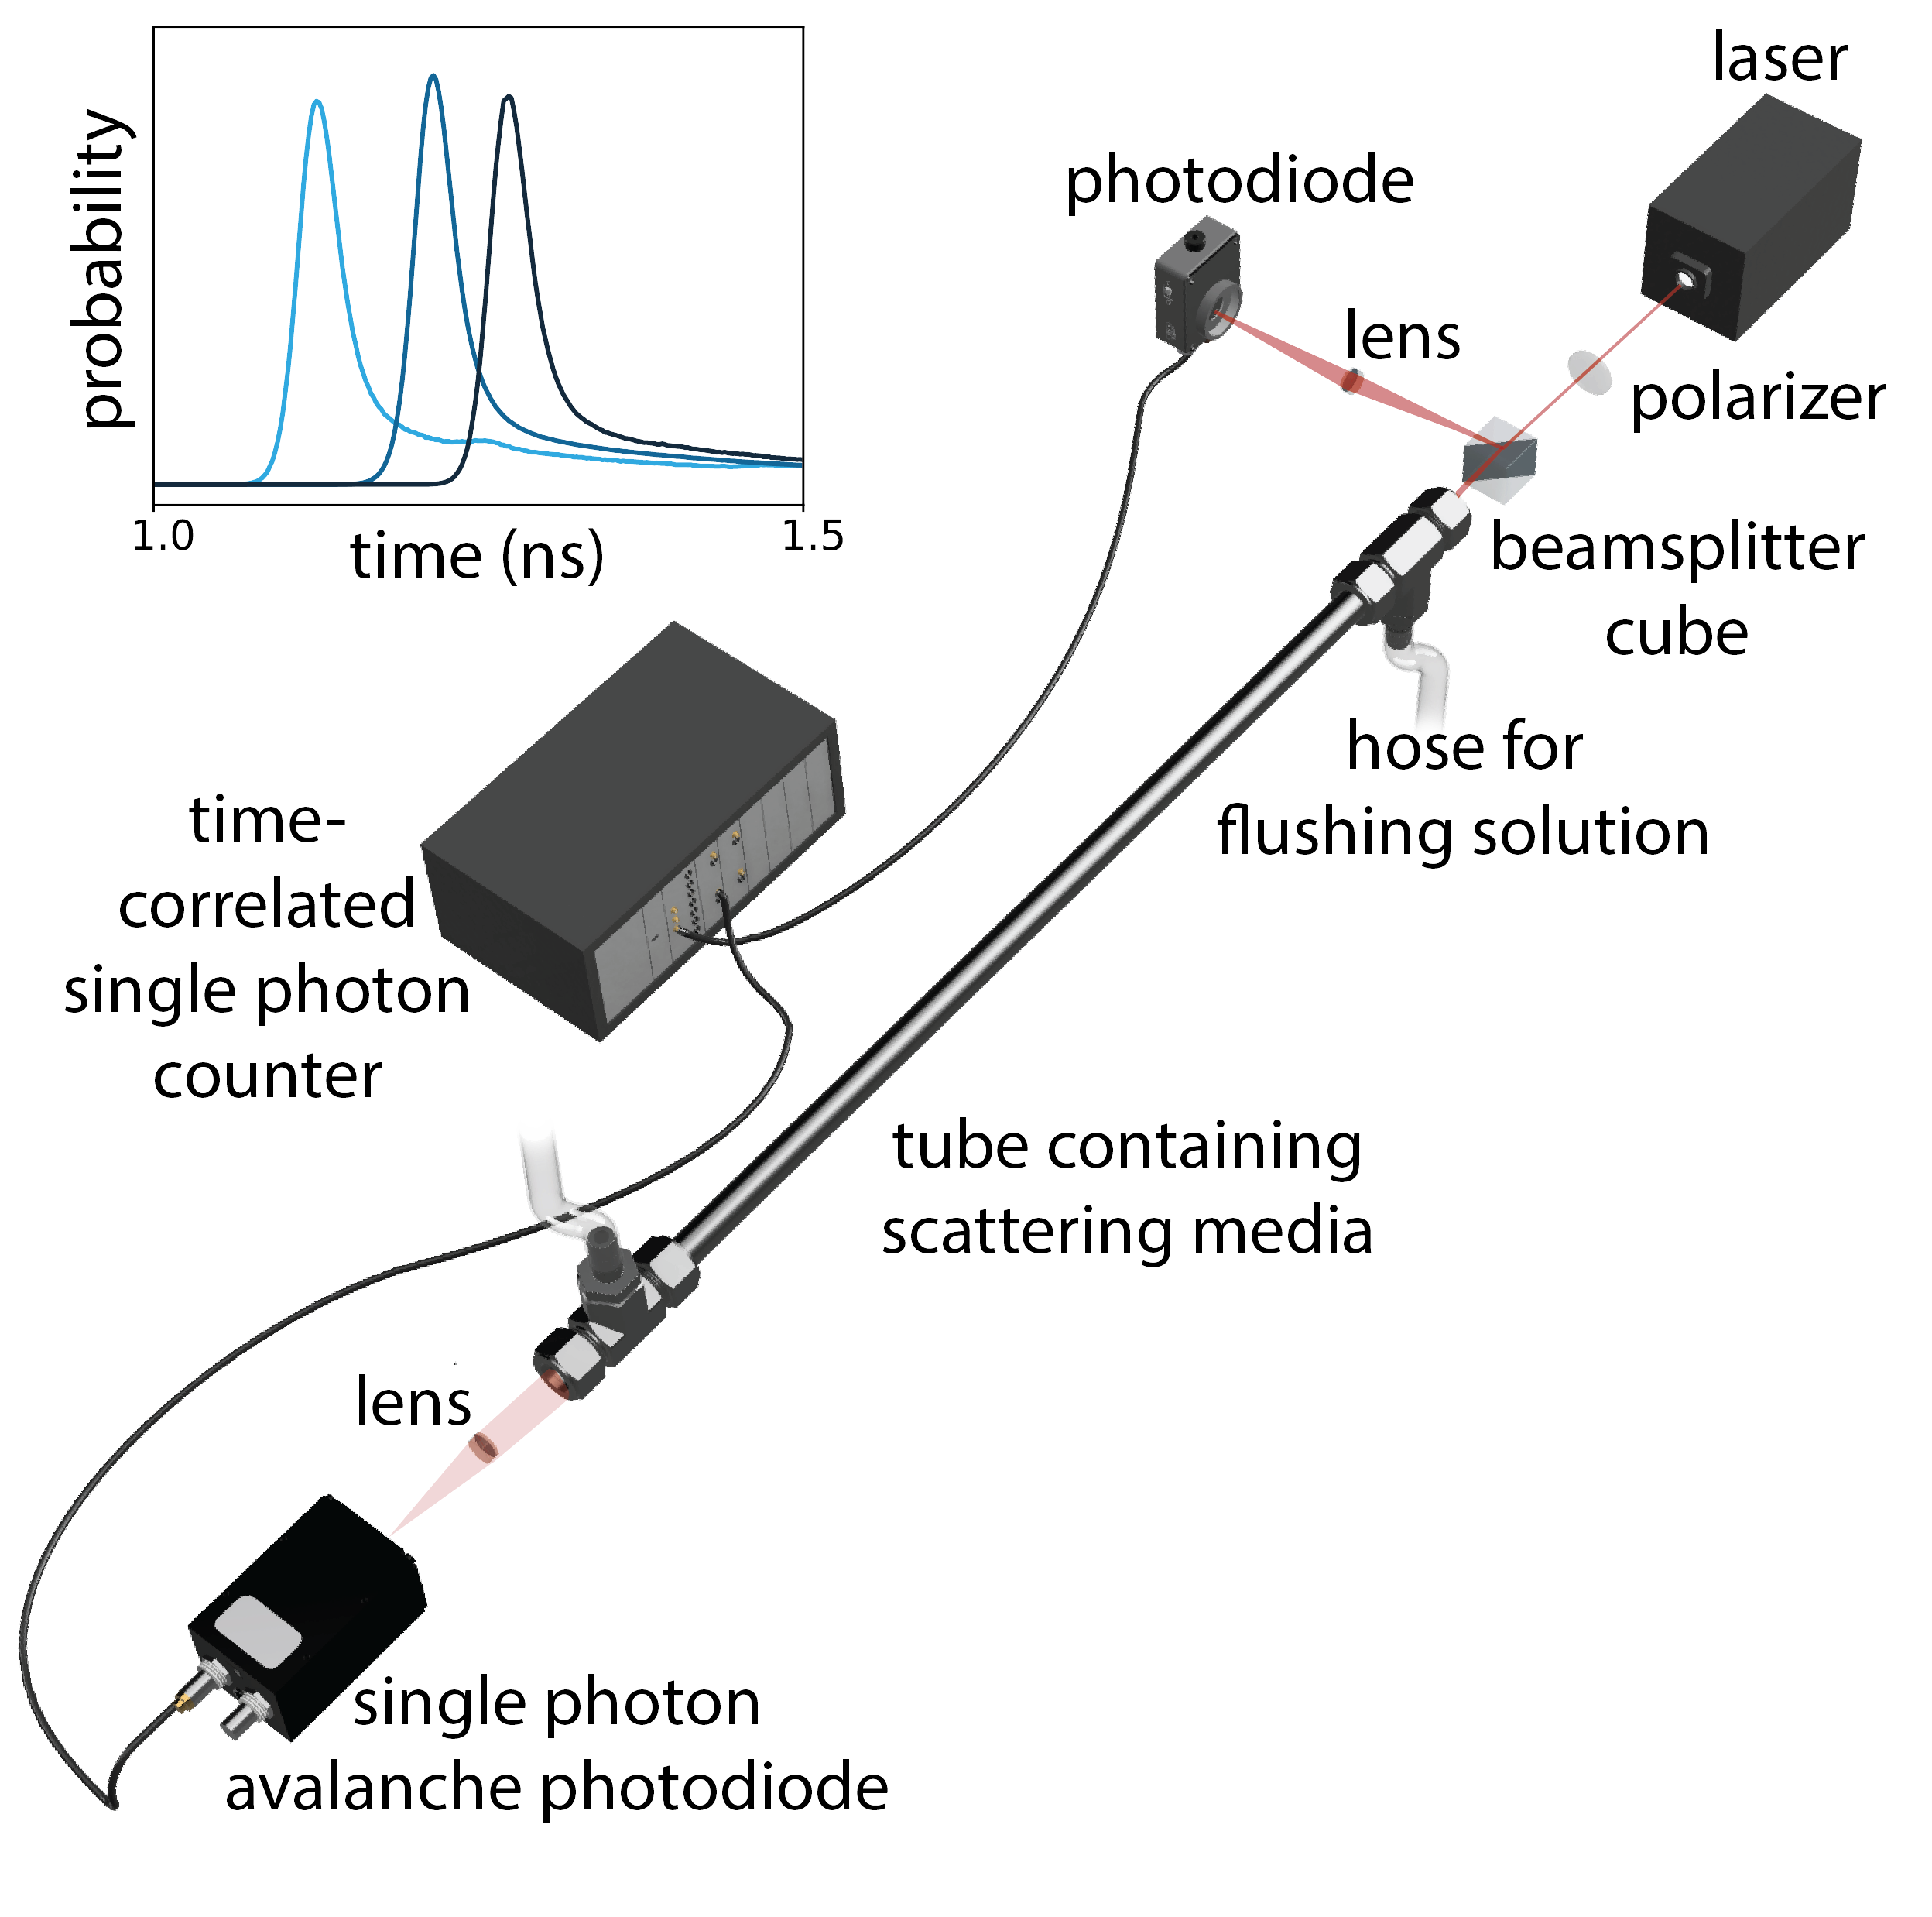
\includegraphics[width=\columnwidth]{images/exp-setup-new.png}
\caption{\label{fig:setup} Experimental setup, consisting of elements described in the text. The signals are collected over an adjustable time period, resulting in a histogram of FPTs. An example of such a histogram at three different concentrations of scattering media is shown, where x axis is the time relative to the speed of light in a vacuum, and the y axis is the probability of that time as the \textbf{first} first arrival.}
\end{figure}


\section{Experimental Methods}\label{sec:exp_meth}

Optical pulses of 140 fs in duration are generated with a femtosecond pulsed laser (Coherent Chameleon Ultra II laser) at frequencies tunable between 680-1080 nm with a repetition rate of 80 MHz and frequency dependent total output power range of 650-3500 mW. These pulses are sent through a power attenuating polarizer (Thorlabs GL10-B).  The majority of the power is bled off through a beamsplitter (Thorlabs BS041) and sent to a photodiode (Thorlabs DET10A).  This photodiode triggers a time-correlated single photon counter (PicoQuant HydraHarp 400) to start a time-of-flight measurement.  The majority of the light continues into a 5/8'' diameter, 1.015 m long stainless steel tube that has been internally polished.  This tube is filled with a solution of water and 10mm silica nanospheres (LUDOX AS-40).  The concentration of nanospheres is tunable, in place, to volume fractions between 0 to 0.235 by flushing the solution and flowing in a new solution.  After travelling through the scattering medium, photons exit the tube and are concentrated through a doublet lens (Thorlabs AC254-030-B-ML) onto a single photon avalanche photodiode (Micro Photon Devices PDM series SPAD).  The signal from the SPAD triggers the photon counter to stop and the time of flight measurement is recorded.  The photon counter and SPAD both have a dead-time less than 80 ns, yielding an effective experimental repetition rate of 12.5 MHz.

The power output varied with wavelength, which made it challenging to discern the number of photons, $N$. The output power varies from 650-3500 mW, and the SPAD detection efficiency varies from 10-30\%.  Factoring in power loss through the optical setup, we find an estimated upper bound of the number $N$ of photons entering the tube as very approximately $10^{12}$.

This experiment uses Ludox AS-40 as a scattering medium because it has a small particle size, scatters strongly, absorbs minimally, is easily diluted with water, and the silica does not aggregate. Ludox has also been well characterized for light scattering purposes\cite{dezelic_determination_1960,bonnelycke_light_1959,goring_light-scattering_1957}. A range of scattering and absorption lengths were produced by diluting Ludox AS-40 in water. Using UV-VIS-NIR spectrometer measurements and the Beer-Lambert law, we determined the absorption coefficient of Ludox AS-40 to be $\sigma_{a}=0.04\ \textrm{m}^{-1}$, which is then multiplied by the concentration to provide the absorption cross section at that concentration. Because the silica nanosphere diameter is roughly 3\% of the wavelengths used in this experiment, the scattering cross section $\sigma_{s}$ was determined via Rayleigh scattering. 


\section{Model Predictions}\label{sec:predictions}

Two common approaches for modelling photon transport are to start with the equation of transfer and make approximations, finding either a diffusion equation or a telegraph equation. Each method is described generally here, resulting in two different photon probability distributions in 1D. We then solve for the probability distribution function of photons located beyond a distance $L$, which, when set equal to $\frac{1}{N}$ for $N$ number of photons, can be solved for the passage time of the first photon of that system to cross that distance. The measured length of the tube $L = 1.015$ m is used, and volume concentrations are determined by the dilution amounts and particle sizes of the Ludox AS-40. Scattering and absorption coefficients, as well as estimated number of photons $N$ are determined as in the Experimental Methods section.


\subsection{Diffusion approximation}\label{subsec:diffusion}

For the diffusion approximation, we look for a solution for the distribution of photons in space and time which satisfies the equation of transfer,
\begin{gather}
    \frac{1}{c} \frac{\partial L \left(\mathbf{r},\hat{s},t\right)}{\partial t} + \mathbf{\nabla} \cdot L\left(\mathbf{r},\hat{s},t\right)\hat{s} = -\left(\sigma_{s} + \sigma_{a}\right) L\left(\mathbf{r},\hat{s},t\right) \notag\\
    \ \ \ \ \ +\ \sigma_{s} \int \int_{4\pi} L\left(\mathbf{r},\hat{s'},t\right) f\left(\hat{s} \cdot \hat{s'}\right) d\Omega' + S\left(\mathbf{r},\hat{s},t\right)\label{eq:RTE}
\end{gather}
which describes the rate in change of radiance $L\left(\mathbf{r},\hat{s},t\right)$ in a given direction $\hat{s}$ and the divergence of radiance from this direction as a sum over any light scattered and absorbed in this direction according to the scattering coefficient $\sigma_{s}$ and absorption coefficient $\sigma_{a}$, any outside light that ends up scattering into this direction, and a source term $S\left(\mathbf{r},\hat{s},t\right)$, with $c$ as the speed of light  \cite{haskell_boundary_1994,ishimaru_wave_nodate}

When the total volume concentration of scatterers greatly exceeds 1\%, a diffusion approximation is often used to describe photon transport. Assuming the diffuse intensity encounters many particles, such that photons scatter almost uniformly in all directions, we can assume a nearly uniform angular distribution \cite{ishimaru_wave_nodate,bohren_absorption_1983}. Neglecting variation and anisotropy in the source term $S\left(\mathbf{r},t\right)$, we can integrate, and in 1D we find
\begin{equation}
    D \partial_{r}^{2} \varphi_{\textrm{diff}} \left(r,t\right) - \sigma_{a} \varphi_{\textrm{diff}} \left(r,t\right) = \frac{1}{c'} \partial_{t} \varphi_{\textrm{diff}} \left(r,t\right) - S \left(r,t\right).
\end{equation}
which is a diffusion equation describing $\varphi_{\textrm{diff}}$ distribution of photons, where $c'$ is the speed of light in the medium \cite{haskell_boundary_1994}. The solution is well known as
a Gaussian multiplied by a decaying exponential for absorption, with a diffusion coefficient dependent on $c'$, $\sigma_{a}$, $\sigma_{s}$, and $g$ the average cosine of the photon scattering angle to account for (an)isotropy.
% \begin{equation}
%     \varphi_{\textrm{diff}}\left(r,t\right) = \frac{1}{\sqrt{4 \pi D t}} \exp\left[{\frac{-r^{2}}{4 D t}-\sigma_{a} t}\right]\label{eq:dif_sol}
% \end{equation}
% where
% \begin{equation}
%     D = \frac{c'}{3\left[ \left(1-g\right)\sigma_{s} + \sigma_{a} \right]}
% \end{equation}
% is the diffusion coefficient, and $g$ is the average cosine of the scattering angle\cite{haskell_boundary_1994,ishimaru_wave_nodate}. 

The FPT distribution for a diffusing particle undergoing a simple symmetric random walk is known to be a Lévy distribution. Thus, the probability that a photon in the diffusion approximation has travelled a distance $L$ at time $t$ is
\begin{align}
     P\left(r \geq L\right) = \frac{\exp\left[{-\sigma_{a} t}\right]}{4 \sqrt{\pi D t}}\textrm{Erfc}\left[{\frac{L}{2 \sqrt{D t}}}\right] \label{FPT_diff}
\end{align}
and when set equal to $\frac{1}{N}$, we solve for $t$ with a given $\sigma_{s}$ scattering coefficient, $\sigma_{a}$ absorption coefficient, and $g$ anisotropy as our extreme FPT for that system.



\subsection{Telegraph equation}\label{subsec:teleg} 
Another way to model photon transport is with a telegraph equation. Beginning with Equation \ref{eq:RTE} and considering photon transport in only one dimension, by following a two-stream approach, or numerous other methods, we can arrive at a telegraph equation for photon transport \cite{schuster_radiation_1905,goldstein_diffusion_1951,durian_two-stream_1996,lemieux_diffusing-light_1998,das_non-fickian_1998,dudko_photon_2005,masoliver_solution_1993,masoliver_finite-velocity_1996,weiss_first_1984,weiss_applications_2002}. The telegraph equation used here is
\begin{align}
     \partial_{r}^{2} \varphi_{\textrm{tel}} \left(r,t\right)  = &\frac{1}{c'^{2}}\partial^{2}_{t} \varphi_{\textrm{tel}}\left(r,t\right) \nonumber \\
     &\ \ + \frac{1}{c'}\left(2 \sigma_{a} + 3 \sigma_{s} \left(1-g\right)\right) \partial_{t} \varphi_{\textrm{tel}}\left(r,t\right) \nonumber \\
    &\ \ \ \ \ \ + \sigma_{a}\left(\sigma_{a} + 3 \sigma_{s} \left(1-g\right)\right) \varphi_{\textrm{tel}} \label{eq:tel}
\end{align}
for $\varphi_{\textrm{tel}}$ concentration of photons \cite{lemieux_diffusing-light_1998}. For short times, this returns the wave equation, and at long times with absorption ignored, we recover the standard diffusion equation with a diffusion coefficient dependent on $\sigma_{s}$ and $g$. This method accounts for the ballistic motion of photons.

From Equation \ref{eq:tel}, we follow the method used in Goldstein (1951) to find the photon distribution
\begin{align}
    \varphi_{\textrm{tel}} \left(r,t\right) &= \frac{1}{2} e^{-\left(\sigma_{a}c' + \gamma \right)t} \bigg[\delta \left(c't - r\right) + \delta\left(ct + r\right) \notag\\
    &\ \ \ \ \ +\left. \Theta\left(c't - |r|\right) \left(\frac{\gamma}{c'}I_{0}\left(\frac{\gamma u}{c'}\right) + \frac{\gamma t}{u}I_{1}\left(\frac{\gamma u}{c'}\right)\right)\right] \label{eq:tel_sol}
\end{align}
where $u=\sqrt{c'^{2}t^{2}-r^{2}}$, and $\gamma = \frac{3}{2} c'\left(\sigma_{s}\left(1-g\right)\right)$ is a time scale determined by the scattering length \cite{goldstein_diffusion_1951,masoliver_solution_1993,masoliver_telegraphers_1994,masoliver_finite-velocity_1996}. We solve for the extreme FPT by integrating Equation \ref{eq:tel_sol} from $L \leq r \leq c' t$, which gives us
\begin{align}
    P\left(r\geq L\right) &=  \frac{1}{2}e^{-\left(\sigma_{a}c' + \gamma \right)t} \int^{c' t}_{L}\bigg[ \delta \left(c't - r\right)  + \delta\left(c't + r\right) \notag\\
    &\left.\ \ \ \ \ + \  \Theta\left(c't - |r|\right) \left(\frac{\gamma}{c'}I_{0}\left(\frac{\gamma u}{c'}\right) + \frac{\gamma t}{u}I_{1}\left(\frac{\gamma u}{c'}\right)\right)\right]  dr \label{FPT_tel}
\end{align}
which we can integrate numerically and solve for $t$, with a given $\sigma_{s}$ scattering coefficient, $\sigma_{a}$ absorption coefficient, and $g$ anisotropy. 

Once we determine the extreme FPTs using Equation \ref{FPT_diff} and \ref{FPT_tel} for given $\sigma_{a}$, $\sigma_{s}$, $c'$, and $g$, we can subtract from them the FPT of light at that wavelength through pure water. This gives us a delay in FPT relative to pure water, and we can observe how that delay changes as scatterer concentration increases.


\begin{figure}[!h]
\includegraphics[width=\columnwidth]{images/lossy-N12-only.pdf}
\caption{\label{fig:alldata} FPT differences measured in the experiment, versus volume concentration. The upper plot is on a linear scale, and the lower plot is on log-log axes. The experimental values are shown as points, the telegraph equation predictions are shown as dashed lines, and the diffusion approximation is shown as dotted lines. Color indicates wavelength, and the solid cyan line is the predicted FPT for a photon travelling through a medium where the index of refraction is averaged for silica and water at that concentration, a value which has negligible variation between these wavelengths.}
\end{figure}



\section{Results and Discussion}

We measured the location of the extreme FPT distribution peak $t$ as a function of scatterer volume concentration $C$. We determined a linear relationship between concentration and extreme FPT peak time, where the extreme FPT peak time matched the predicted passage time of light passing through an index-averaged medium, independent of wavelength. The data are shown in Figure \ref{fig:alldata}.

We collected a range of FPT distributions at a range of wavelengths. Integration times ranged from 1-300 seconds, and this did not affect the results. The extreme FPT difference comes from subtracting the extreme FPT through pure water $t\left(0\right)$ from the peak FPT at a given volume concentration of scatterers $t\left(C\right)$, by wavelength to remove any error introduced by inconsistencies in the laser at different wavelengths. The line and point color in Figure \ref{fig:alldata} indicates the light wavelength, and the concentration $C$ is given by volume fraction. There does not appear to be a wavelength dependence for the measured extreme FPT difference. At full Ludox AS-40, or volume fraction of $C$ = 0.235, the measured difference in extreme FPT is 0.111 ns, or 111 ps. 

The diffusion approximation yields extreme FPTs that are nonphysical, predicting photons that travel faster than the speed of light, for scatterer volume concentrations $C$ below around 3 \% for 680 nm and 6.3 \% for 830 nm. Beyond these concentrations, the predicted extreme FPT increases linearly with concentration for both wavelengths, reaching over 31,000 ps and 12,200 ps for 680 nm and 830 nm respectively at 0.235 scatterer volume concentration. 
The telegraph equation method predicts a linear relationship for extreme FPT delay which is related to the speed of light in the index-averaged medium. Upon reaching around 0.01175 (680 nm) or 0.0235 (830 nm) volume concentration, we begin to expect a stronger delay. For 680 nm we find a delay of 16,667 ps at 0.049 volume concentration, and for 830 nm we get a delay of 8,048 ps at 0.057 volume concentration. Beyond this point, the loss from scattering and absorption cause all $N$ photons to leave the system before reaching $L$ = 1.015 m {\color{violet}(is this the right explanation?)}. Rayleigh scattering is isotropic in the forward and backward directions, so we set $g=0$ \cite{bohren_absorption_1983}. For both approximations, there is significant wavelength dependence. Dotted line curves in Figure \ref{fig:alldata} show the diffusion approximation results, and dashed lines show the telegraph equation results.

The diffusion model does not accurately describe first first passage photons, as it either violates causality or predicts a far-too-long lag in extreme FPTs. In order to recreate the measured values for the telegrapher model, with wavelength-independent results in isotropic scattering conditions for all concentrations, $N \approx 10^{117}$ photons are required entering the tube. The number of photons in the universe are around $10^{89}$. For the telegraph predictions to fit the data in the maximum case of $N=10^{12}$ photons, the anisotropy factor would have to be approximately $g = 0.972$. For decreasing N, the required anisotropy factor increases, until eventually $g=1$, representing forward-scattering conditions, is required for a lower bound of $N=10^{3}$ photons to achieve the measured extreme FPT, which is wavelength-independent and matches the index-averaged time (really bad run-on sentence). Lower $N$ values do not achieve any of the measured extreme FPT differences. With 20 nm spheres and 680-730 nm light, it is incorrect to assume forward-scattering behavior for the bulk of the photons - $g$ should be much closer to 0. Given these factors, the telegraph equation solution also does not accurately describe first first passage photons.

% The output power is lowest at the lowest wavelength, 680 nm, and because passing through the optics in the light path attenuates this power further, we end up with power in the $\textrm{\mu}$W range or lower. Additionally, the SPAD detection efficiency decreases over this range, dropping to around 10-15 \% at 830 nm. The average power entering the tube is anywhere from 0-0.5 $\textrm{\mu}$W at 720 nm, where the laser power and SPAD quantum efficiency combine to generate the highest input count rate at the detector. Accounting for the energy of photons at that wavelength, we find an estimated upper bound of the number $N$ of photons entering the tube as very approximately $5 \times 10^{12}$. Using $N=10^{12}$ will give us a lower bound on predicted extreme FPTs from the models, because with decreasing $N$, the extreme FPT time would simply increase.


\section{Conclusion}
We have measured the relationship between photon extreme FPT and scatterer volume concentration, finding a significantly different relationship than that predicted by either the diffusion approximation or the telegraph equation for radiative transport. Rather than matching the predictions from these models, the extreme FPTs correspond with the time it takes a photon to travel through an index-averaged medium. These models therefore do not appropriately describe the underlying physics. While they often predict the behavior of the average photon travelling through scattering media and can be used to infer bulk properties, they cannot be used to understand the extreme photons, or to reveal underlying correlated behavior in the environment. A model that accounts for these extreme first passage photons moving ballistically would more accurately describe the underlying physical process, and in turn, open up the possibility that the extreme FPT statistics could uncover important information about the diffusive environment, with applications in many areas of science as a whole \cite{allgaier_diffuse_2021, collis_lidar_1966, loumaigne_intrinsic_2015, aleandri_dynamic_2018, taitelbaum_diagnosis_1999,das_non-fickian_1998,weiss_applications_2002,dudko_photon_2005}.

\section{Acknowledgments}
We thank M. Allgaier, J. Hass, and R. Parthasarathy for discussions. This work was funded under the W. M. Keck Foundation Science and Engineering grant on “Extreme Diffusion.”
\bibliographystyle{unsrt}
\bibliography{paper_bib}

\end{document}